\documentclass[border=5pt]{standalone}
\usepackage{tikz}
\begin{document}
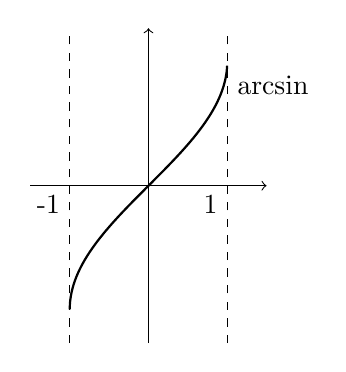
\begin{tikzpicture}
\draw [->] (0,-2)-- (0,2);
\draw [->] (-1.5,0) -- (1.5,0);
\draw [thick, smooth, samples = 1000, domain=-1:1] plot (\x, {asin(\x)/180*pi}) node [below right] {$\arcsin$};
\draw [dashed] (-1,-2) -- (-1,2);
\node [below left] at (-1,0) {-1};
\draw [dashed] (1,-2) -- (1,2);
\node [below left] at (1,0) {1};
\end{tikzpicture}
\end{document}
